\chapter{Umsetzung der Anwendung}
\thispagestyle{fancy}
Im folgenden soll die Umsetzung der Anwendung thematisiert werden. Umsetzung meint hier sowohl die Programmierung der Anwendung und alle Bereiche, die mit dieser zusammen hängen, als auch die visuelle Gestaltung. Dieses Kapitel geht auf Konzepte ein, die währen der Gestaltung der Anwendung eine zentrale Rolle spielten und schildert das generelle Vorgehen. Es werden einige strukturelle Entscheidungen erläutert, die währen der Umsetzung von Relevanz waren und einige konkrete Codebeispiele gezeigt, die als besonders interessant erachtet wurden.

\section{Gestaltung}
Bereits in Kapitel \ref{sec:relevance} wird deutlich, welche zentrale Rolle die Gestaltung in jedwedem Projekt einnimmt. Auch das hier bearbeitete Projekt ist davon nicht ausgenommen. Um eine gute Benutzbarkeit des Tools zu gewährleisten, ist eine solide Gestaltung unabdingbar.\\
Steve Krug schreibt über die Gestaltung von Webseiten:

\begin{quote}
  Die Seiten offensichtlich zu gestalten, ist wie eine gute Beleuchtung in einem Geschäft: Alles erscheint einfach besser. Die Nutzung einer Website, die uns nicht zum Nachdenken über Unwichtiges zwingt, fühlt sich mühelos an, wogegen das Kopfzerbrechen über Dinge, die uns nichts bedeuten, Energie und Enthusiasmus raubt — und Zeit. \cite[S. 19]{Krug201410}
\end{quote}

Insgesamt ist \textit{25knots} eine sehr interaktive Anwendung, in der Informationen eher Grafisch und durch Interaktionen des Benutzers übertragen werden, als Beispielswiese durch Texte.
Daher wurde bei der Gestaltung großer Wert darauf gelegt, klar zu kommunizieren, welche Bereiche interaktiv sind und welche Auswirkungen eine Interaktion mit diesen Bereichen hat.\\
Um diese Abgrenzung zu gewährleisten, wurde ein schlichtes Farbschema verwendet, in dem nur zwei Farben, Blau und Rot, verwendet wurden, die zur Anzeige von Interaktivität dienen.
Die beiden Farben haben dabei festgelegte Rollen: Blau zeigt Interaktivität innerhalb eines Schrittes der Anwendung an, Rot zeigt zwischen verschiedenen Schritten übergreifende Aktivitäten an. Abbildung \ref{fig:entrance} zeigt die Ausführung dieser Idee am Beispiel des Einstiegs in die Anwendung. Die blauen Elemente erlauben eine Auswahl innerhalb des Einstiegs (nächster Zwischenschritt, Auswahl eines Entwicklungsziels), der rote Button am unteren Rand erlaub das wechseln zum nächsten Abschnitt in der Anwendung.

\begin{figure}[h]
    \centering
    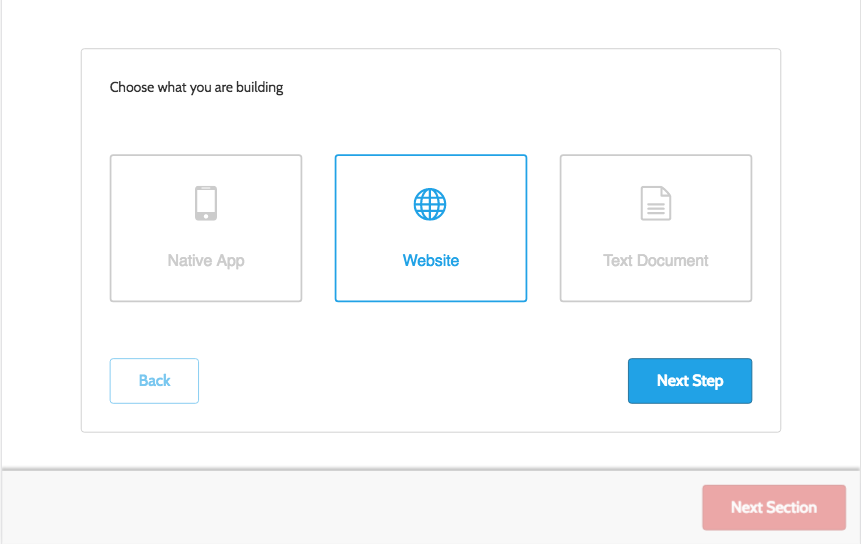
\includegraphics[width=1\textwidth]{images/25knots_entrance.png}
    \caption{Farben verschiedener interaktiver Elemente}
    \label{fig:entrance}
\end{figure}

Weiterhin gilt es zu beachten, dass der Nutzer die Anwendung verwendet, um eine Gestaltung für sein Projekt zu erstellen. Der Fokus der Anwendung sollte daher darauf liegen, dem Nutzer die von ihm erarbeitete Gestaltung zu zeigen. Die Anwendung selbst sollte sich nur in bestimmten Fällen (beispielsweise beim Auftreten eines Fehlers oder wenn eine Interaktion notwendig ist) in den Vordergrund stellen. Daher wurde darauf geachtet, die Anwendung so simpel wie möglich zu gestalten und auf unnötige gestalterische Experimente zu verzichten. Der größte Teil der Anwendung ist in Weiß- und Grautönen gehalten, um die Gestaltung des Nutzers und dessen Entscheidungen besser in den Vordergrund stellen zu können.

Dieses Vorgehen lässt sich anhand von zwei Beispielen gut verdeutlichen.\\
Zum Einen seien hier die Fehlermeldungen im Bereich Typographie genannt. Diese sind in einem auffälligen Gelb hinterlegt, dass nur für diesen bestimmten Anwendungsfall (das hervorheben von Fehlern) verwendet wird und dem Nutzer dadurch schnell auffällt (siehe Abbildung \ref{fig:warning}).
Zum Anderen zeigt die Auswahl von Farben (vor allem in den \textit{scopes} Android und iOS) gut, wie Interaktive Elemente in der Anwendung bereits die Gestaltung des Nutzers zeigen können. Die Buttons zur Auswahl einer Farbe (siehe Abbildung \ref{fig:accent}) bestehen hier lediglich aus der Farbe selbst, die Anwendung und deren Gestaltung wird hier als visuelle Zwischenebene komplett entfernt.

\begin{figure}[h]
    \centering
    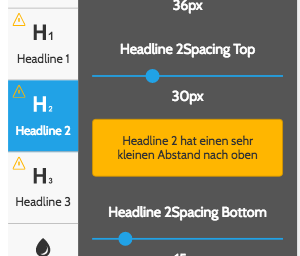
\includegraphics[width=0.5\textwidth]{images/25knots_Warning.png}
    \caption{Fehlermeldungen im Bereich Typographie}
    \label{fig:warning}
\end{figure}

\begin{figure}[h]
    \centering
    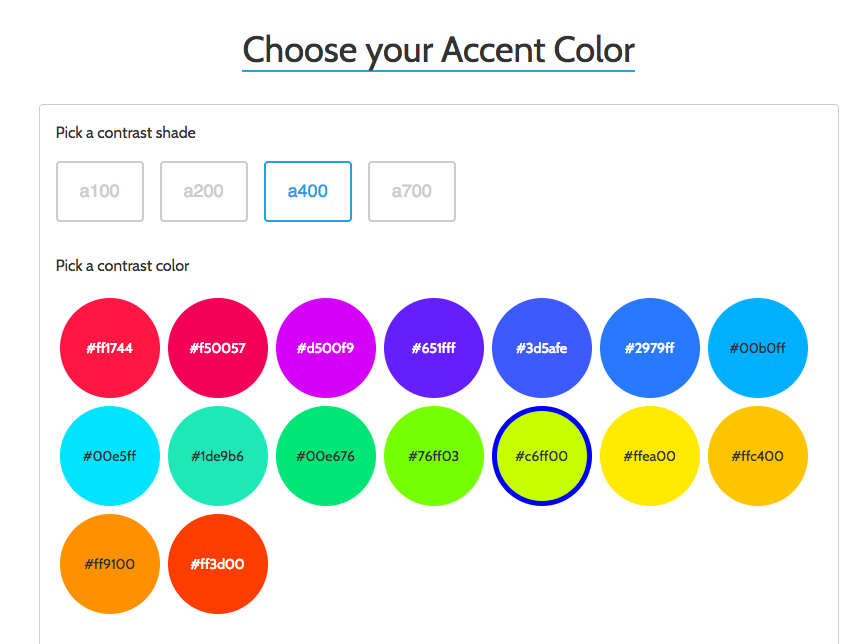
\includegraphics[width=1\textwidth]{images/25knots_color_button.png}
    \caption{Buttons zum Auswählen einer Akzentfarbe}
    \label{fig:accent}
\end{figure}


\subsection{Vorgehen}
Das Vorgehen während der Gestaltung lässt sich als \textit{agil} bezeichnen. Diese Agilität drückt sich auf verschiedene Weise aus.\\
Der Entwicklungsprozess (gemeint ist hier die tatsächliche Programmierung) und der Gestaltungsprozess (das Erstellen von Mock-Ups in einem entsprechenden Grafikprogramm) waren nicht strikt von einander getrennt, sondern überschnitten sich. Diese Überschneidung zeigt sich sowohl in einer langfristigen, als auch in einer kurzfristigen Betrachtung.\\
So gab es nicht einen Gestaltungsprozess, nach dessen Fertigstellung die Entwicklung startete, sondern vielmehr einen Gestaltungsprozess pro Schritt der Anwendung, der umgesetzt wurde.\\
Auch innerhalb eines Schrittes war das Vorgehen nicht linear, häufig wurden während der Entwicklung Aspekte in der Gestaltung verändert. Die Gründe hierfür liegen vor allem in den verbesserten Möglichkeiten zum testen und validieren von Interaktionen und Konzepten in einer prototypischen Realisierung im Vergleich zu statischen Mock-Ups.
Durch die in Kapitel \ref{chap:spacing} und \ref{chap:styleguide} erläuterten Aspekte konnten außerdem problemlos kleinere Änderungen in der Gestaltung während der Entwicklung vorgenommen werden, ohne, dass dabei ein vorheriges Anpassen der Mock-Ups nötig war.

\subsection{Abstände}
\label{chap:spacing}
Um den Gedanken von innerhalb der Anwendung wiederverwendbaren Komponenten zu unterstützen liegt der Gedanke nahe, auch Abstände innerhalb der Gestaltung (und später auch in der Umsetzung) wiederverwendbar zu entwerfen. Die Grundlage für diesen Gedanken lieferte ein Artikel von Nathan Curtis \cite{CurtisSpace16}. Der Artikel enthält zwei Grundgedanken:

\begin{enumerate}
  \item Die Größen von Abständen sollten sollten festgelegt und ihre Anzahl übersichtlich sein.
  \item Es gibt verschiedene Arten von Abständen, die die verschiedenen Größen auf unterschiedliche Weise einsetzen und kombinieren.
\end{enumerate}

Diese Gedanken wurden in der Gestaltung und Umsetzung des Projektes übernommen. Zunächst wurden die verschiedenen Abstände, aufbauend auf der von Curtis empfohlenen Basisgröße von 16px, definiert. Aufbauend auf der Basisgröße wurden anschließend Abstufungen in beide Richtungen
Erstellt, die nach Kleidergrößen, von XS bis XXL, benannt wurden.
Diese Abstufungen wurden in einer eigenen Datei als JavaScript-Objekt deklariert, so dass über die gesamte Anwendung hinweg diese festgelegten Größen verwendet werden können.

\begin{figure}[h]
    \centering
    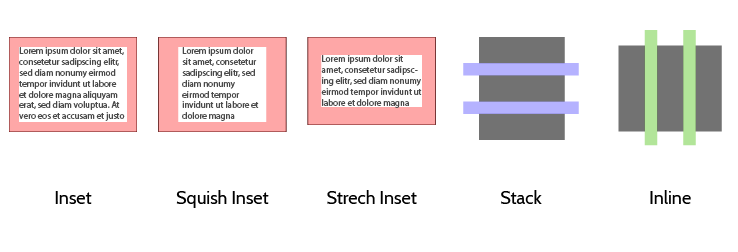
\includegraphics[width=1\textwidth]{images/spacing_types.png}
    \caption{Die 5 implementierten Arten von Spacing nach \cite{CurtisSpace16}}
    \label{fig:spacing}
\end{figure}


Curtis definiert 6 verschieden Arten von Abständen, von denen 5 innerhalb der Anwendung als eigenständige Komponenten definiert wurden (siehe Abbildung \ref{fig:spacing}).\\
Die Komponenten nehmen die Größe des Abstandes als \verb|prop| in einer der definierten Kleidergrößen entgegen und erzeugen ein \verb|div| Element, das die Abstände als \verb|padding| oder \verb|margin| anwendet.
Die Pixelwerte für die jeweilige Abstandsgröße erhält die Komponente dabei durch den Aufruf des für die Abstandsgrößen zuständigen JavaScript-Objekts (zum Beispiel \verb|spacing.l|). Alle diese Komponenten rendern außerdem die ihnen übergebenen Kinder, sodass eine Verwendung der \verb|SpacingInset| Komponente wie in Listing \ref{lst:spacingInset} möglich wird.

\begin{lstlisting}[caption=Beispielhafte Verwendung einer Komponente für Abstände, label=lst:spacingInset]
  <SpacingInset size='l' >
    <h1> A Headline </h1>
    <p> Some Text </p>
  </SpacingInset>
\end{lstlisting}

Hier stellt sich die Frage, inwiefern es Sinn ergibt, Komponenten zu definieren, die eine ausschließlich visuelle Funktion haben.
So könnte deren Funktion auch innerhalb der CSS-Regeln von anderen Komponenten definiert und so ein übersichtlicheres Markup geschaffen werden.\\
Während der Arbeit stellte sich heraus, dass die Definition er Abstände als eigene Komponenten ein sehr einfaches Entwickeln von Interfaces ermöglichte. Durch die eingegrenzten Möglichkeiten ist auch währen der Entwicklung ein testen von anderen Abständen sehr einfach möglich.\\
Weiterhin ist der Raum für Inkonsistenzen begrenzt, da die Abstände nur in den vorgegebenen Größen angegeben werden können. Dies wurde, gerade mit Blick auf die spätere Weiterentwicklung und Veröffentlichung, als ausreichend großer Vorteil angesehen, um eine Definition als eigenständige Komponente zu rechtfertigen.

\subsection{Styleguide}
\label{chap:styleguide}
Da zu einem späteren Zeitpunk unter Umständen verschiedene Personen an der Weiterentwicklung der Anwendung beteiligt sein werden, macht das Festhalten der bisher gestalteten Elemente und der Grundlagen der Gestaltung durchaus Sinn.
Während der Gestaltung wurde nur ein minimalistischer Styleguide mit Informationen über Farben, Schriftgrößen und Abstände geführt, der für die Gestaltung dieser ersten Version mit nur einer Person im Team ausreichend war.

Mit Blick auf die spätere Weiterentwicklung ist ein Zentraler Ort, der einen Überblick über die bereits erstellten Komponenten gibt, von großem Vorteil.
Hierfür wurde die Bibliothek Storybook\footnotemark{} verwendet. Die Bibliothek wird lokal im Browser ausgeführt und ermöglicht es, verschiedene Komponenten aus der Anwendung gekapselt darzustellen. Hierbei ist kein doppelter Code notwendig, die Komponenten können direkt aus dem Anwendungscode übernommen werden.
Die Bibliothek bietet dadurch außerdem den Vorteil, dass Komponenten zunächst alleinstehend entwickelt werden können, ohne dass diese in die eigentliche Anwendung eingebunden werden müssen.

\footnotetext{\url{https://github.com/storybooks/storybook}}

\section{Redux}
\label{chap:redux}

Im laufe der Anwendung müssen bestimmte Informationen über die gesamte Anwendung hinweg für bestimmte Komponenten abrufbar sein. Dies betrifft vor allem, aber nicht ausschließlich, die vom Nutzer zu beginn der Interaktion mit der Anwendung definierten Entwicklungsziele, die in jedem Bereich der Anwendung für die korrekte und auf das jeweilige Ziel angepasste Darstellung der  Inhalte überprüft werden.\\
Ein weiteres Beispiel stellt die Zusammenfassung am Ende der Interaktion mit der Anwendung dar, für die ein Zugriff auf alle vom Nutzer definierten Werte nötig ist. Der Redux-Store für die Anwendung umfasst daher Werte aus den Bereichen \textit{Intro}, \textit{Typographie} und \textit{Farben}.\\

Um die Arbeit mit dem Store zu simplifizieren und eine übermäßige Ver­schach­te­lung des Store-Objekts zu vermeiden, wurde für jeden der oben genannten Bereiche ein eigener \textit{Reducer} geschrieben, der ausschließlich für die Bearbeitung der diesem Bereich zugehörigen Werte verantwortlich ist.\\
In der Datei \verb|ApplicationState.js| werden diese mit Hilfe der Funktion \verb|combineReducers|, die von Redux zur Verfügung gestellt wird, dann zu einem Objekt zusammengefügt (siehe Listing \ref{lst:combine_reducer}).

\begin{lstlisting}[caption={Zusammenfügen der dedizierten Reducer zu einem Objekt}, label=lst:combine_reducer]
  const ApplicationState = combineReducers({
    setup: setup,
    typography: typography,
    colors: colors
})
\end{lstlisting}

\subsection{Beispielhaftes Verändern des Redux-Store}
Das Verändern des Redux-Store soll im Folgenden an einem konkreten Beispiel verdeutlicht werden. Das Szenario, das der Nutzer durchläuft, ist dabei das Auswählen einer Grundfarbe. In diesem Szenario hat der Nutzer bereits eine Wahl über seine Grundfarbe getroffen und möchte nun durch den Klick auf den \textit{Next Step} Button seine Auswahl bestätigen und zum nächsten Schritt übergehen (vergleiche hierzu Abbildung \ref{fig:colors_bg} auf Seite \pageref{fig:colors_bg}).\\
Für die Anwendung bedeutet diese Interaktion: Die aktuell gewählte Grundfarbe muss in den Redux-Store geschrieben\footnotemark{} und der nächste Schritt für die Farbfindung angezeigt werden. Dieses Beispiel soll sich dabei auf das schreiben der Grundfarbe in den Redux-Store konzentrieren.\\

Um diese Veränderung im Redux-Store möglich zu machen, muss zunächst eine \textit{action} definiert werden (Listing \ref{lst:action}), auf deren Aufrufen hin der \textit{reducer} (Listing \ref{lst:reducer}) den Redux-Store aktualisiert.

\footnotetext{Es ist dabei möglich, dass mehr als eine Grundfarbe gespeichert wird, da für das Zielmedium Android insgesamt drei Abstufungen einer Grundfarbe benötigt werden.}

\begin{lstlisting}[caption={Definition der \textit{action} zum setzen der Grundfarben}, label=lst:action]
  export const setBaseColors = (colors) => {
    return {
      type: SET_BASE_COLORS,
      colors
    }
  }
\end{lstlisting}

\begin{lstlisting}[caption={Veränderung des Redux-Store beim Aufrauf der \textit{action} \texttt{setBaseColors}}, label=lst:reducer]
  case SET_BASE_COLORS:
    return Object.assign({}, state, {
      baseColors: [
        ...action.colors
      ]
    })
\end{lstlisting}

Die \textit{action} kann innerhalb der Anwendung durch den Aufruf der Methode \verb|dispatch(setBaseColors(colors))| ausgelöst werden. Der Aufruf dieser Methode ist theoretisch direkt in der Komponente die den Button definiert, auf den der Nutzer klickt, möglich. Dieses Vorgehen wäre allerdings nicht mit den in Kapitel \ref{chap:component} definierten Anforderungen an eine Komponenten konform. So könnte dieser Button nur an Stellen eingesetzt werden, an denen die Grundfarbe für den Bereich Farben im Redux-Store gesetzt werden soll (realistisch betrachtet würde diese Komponente also an genau einer Stelle eingesetzt werden).\\
Um diesen Umstand zu vermeiden, wird die Methode als Referenz weiter gegeben (Abbildung \ref{fig:redux_flow} zeigt eine informelle Darstellung aller beteiligter Komponenten).

\begin{figure}[h]
    \centering
    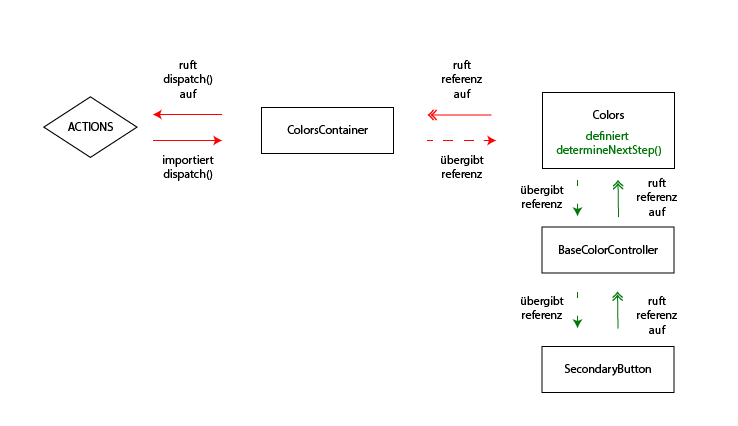
\includegraphics[width=1\textwidth]{images/redux_store_flow.png}
    \caption{Übergabe der \texttt{dispatch()} Methode als Referenz}
    \label{fig:redux_flow}
\end{figure}

In der Komponente \textit{ColorsContainer} wir die Referenz auf die \verb|dispatch()| Methode als \verb|prop| mit dem Namen \verb|setBaseColors| an die Komponente \textit{Colors} übergeben.

Die Komponente \textit{Colors} implementiert die Funktion \verb|determineNextStep|, die Feststellt, welcher Schritt in Abhängigkeit vom Entwicklungsziel des Nutzers der nächste ist. Die Referenz auf \verb|setBaseColors| wird dabei auf jeden Fall aufgerufen. Die Komponente \textit{Colors} gibt nun eine Referenz auf die Funktion \verb|determineNextStep| an die Komponente \textit{BaseColorController} weiter. Diese wiederum gibt diese Referenz an die Komponente \textit{SecondaryButton} weiter, die auch die Komponente ist, mit der der Nutzer interagiert.

Die \textit{SecondaryButton} Komponente führt auf einen Klick die ihr als \verb|prop| übergebene Referenz auf eine Funktion aus (siehe Listing \ref{lst:sec_btn}) und hat selbst kein Wissen darüber, welche Funktion innerhalb der Anwendung sie ausführt. Hierdurch werden die übergebenen Referenzen in rückläufiger Reihenfolge wieder aufgerufen und so der \verb|dispatch()| ausgelöst.

\begin{lstlisting}[caption={Aufruf der übergebenen Funktion in der Komponente \textit{SecondaryButton}}, label=lst:sec_btn]
  function SecondaryButton(props) {
    return (
      <button
        className={setStyles(props.variant, props.inactive)}
        onClick={props.inactive ? '' : props.onClick}
      >
        <SpacingSquishedInset size='l'>
          {props.children}
        </SpacingSquishedInset>
      </button>
    )
}
\end{lstlisting}

\section{CSS-Architektur}
In der Entwicklung von Webanwendungen wird es als gutes Vorgehen angesehen, Inhalte und deren Gestaltung voneinander zu trennen \cite[S. 56]{goodman2002dynamic}. Diese Trennung erfolgt in der Regel durch das definieren von dedizierten HTML- und CSS-Dateien, die sich nur mit der Struktur von Inhalten bzw. deren Aussehen befassen.
Eine der aktuell verbreitetsten Möglichkeiten, Regeln für die Darstellung von Inhalten zu definieren, ist das vergeben von Klassen über das \verb|class|-attribut, die dann in der CSS-Datei über einen Selektor (zum Beispiel \verb|.myClass|) aufgerufen werden können.

Auch React.js bietet die Möglichkeit, diese Architektur abzubilden. In Kapitel ZXC wurde bereits erwähnt, dass hier wegen der Verwendung von JavaScript in Komponenten das Attribut \verb|className| verwendet werden muss.

Durch die Verwendung einer solchen Architektur werden für Komponenten jedoch Abhängigkeiten geschaffen, da für die korrekte Darstellung der Komponente auch immer die entsprechenden Regeln in der CSS-Datei verfügbar sein müssen.
Diese Abhängig von ihrer Umwelt ist jedoch nicht Konform mit den in Kapitel AZS definierten Anforderungen an eine Komponente innerhalb dieser Arbeit.

Um das Aussehen innerhalb von HTML-Elementen zu verändern, kann das \verb|style|-attribut verwendet werden. Auch dieses akzeptiert CSS-Syntax, die das Aussehen des jeweiligen Elements definiert.
React.js ermöglicht die Verwendung dieses Attributes innerhalb von Komponenten und somit auch die Deklaration von Inhalt und Aussehen innerhalb einer Komponenten, ohne die Notwendigkeit weiterer Abhängigkeiten.

Die Verwendung des \verb|style|-attributes zum Festlegen des Aussehens birgt jedoch einige Nachteile. So können über das Attribut keine Pseudo-Klassen, wie zum Beispiel \verb|:hover| oder \verb|:before| angesprochen werden. \cite{w3c2017styles}
Für die Entwicklung der Anwendung sind die Pseudo-Klassen jedoch notwendig.
Um dieses Problem zu lösen, wurden im Bereich der \textit{JavaScript-SPAs} viele Bibliotheken entwickelt. Im Rahmen dieses Projektes wurde die Bibliothek Aphrodite\footnotemark{} verwendet.
Diese Bibliothek erlaubt eine Notation der CSS-Regeln wie sie React.js auch nativ ermöglicht, unterstützt aber beispielsweise Pseudo-Klassen (Listing \ref{lst:aphro} zeigt ein simples Beispiel).

\footnotetext{\url{https://github.com/Khan/aphrodite}, zuletzt abgerufen am 12.08.2017}

\begin{lstlisting}[caption=Beipspielhafte Verwendung der Bibliothek Aphrodite, label=lst:aphro]
	import React from 'react'
	import { StyleSheet, css } from 'aphrodite'

	function myComponent(props) {
		<div className={css(styles.componentStyles)} >
			{props.children}
		</div>

		const styles = StyleSheet.create({
			componentStyles: {
				color: 'blue',
				':hover': {
					color: 'red'
			}
		})
	}
\end{lstlisting}

Während der Entwicklung wurde nicht jegliche Art von Gestaltung innerhalb von Komponenten realisiert. Verschiedene native HTML-Elemente, die über die Anwendung hinweg verwendet werden, wurden in einer globalen CSS-Datei definiert. Dies hat den Vorteil, dass zum Beispiel für die Verwendung einer Überschrift keine eigene Komponente geschrieben werden muss, die funktional equivalent zu einem nativen HTML-Element (beispielsweise \verb|<h1>|) ist, nur um dessen Aussehen anzupassen.

\section{Interessante Aspekte in der Entwicklung}
Nachfolgend sollen einige konkrete Beispiele aus der Entwicklung der Anwendung erläutert werden. Die verschiedenen Beispiele wurden dabei aus unterschiedlichen Gründen Gewählt:
Kapitel \ref{chap:state_component} zeigt einen zentralen Aspekt der Umsetzung einer komponentenbasierten Anwendung mit React.js, Kapitel \ref{chap:display_scope} eine der zentralen Arbeitsweisen der Anwendung. Die Kapitel \ref{chap:colors_dev} und \ref{chap:pdf} zeigen die Lösung von Problemen, die für die Funktionalität der Anwendung eine hohe Relevanz besitzen.


\subsection{State in Komponenten}
\label{chap:state_component}
Das Konzept des \textit{state} in React.js wurde Bereits in Kapitel \ref{chap:stateless} angesprochen. Hier soll an einem konkreten Bespiel verdeutlicht werden, wie der \textit{state} genutzt werden kann, um auf Nutzereingaben zu reagieren und an inwiefern sich der Zustand einer Komponente vom Zustand der gesamten Anwendung unterscheidet.
Als Beispiel wurde die Auswahl des Zielmediums durch den Nutzer im ersten Schritt der Anwendung gewählt, die in mehreren Schritten durchgeführt wird.
Der Ablauf der Interaktion mit der Anwendung sieht dabei wie folgt aus:
Die Anwendung präsentiert dem Nutzer drei Optionen, aus denen dieser wählen kann. Wählt der Nutzer eine der Optionen aus, gibt die Anwendung ihm eine visuelle Rückmeldung über die ausgewählte Option. Ist der Nutzer mit seiner Wahl zufrieden, bestätigt er diese durch einen Button und  ihm wir der nächste Schritt im Wizard angezeigt.

Für diese Interaktion werden verschiedene Komponenten eingesetzt (siehe dazu Abbildung \ref{fig:components}), von denen die meisten \textit{stateless} sind, lediglich die Komponente \verb|SetupProgress|, die in Listing \ref{lst:setup} zu sehen ist\footnotemark{}, verwaltet einen Zustand.

\begin{figure}[h]
    \centering
    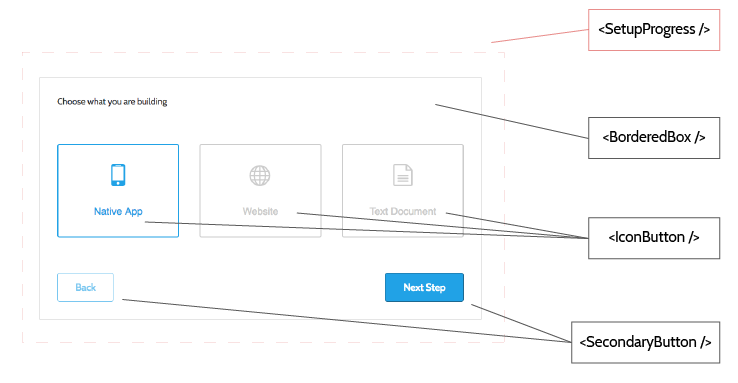
\includegraphics[width=1\textwidth]{images/components.png}
    \caption{Komponenten im der Festlegung des Zielmediums}
    \label{fig:components}
\end{figure}

\footnotetext{Teile des Quellcodes, die für diesen Anwendungsfall nicht relevant sind, wurden gekürzt. Die gesamte Datei kann der beiliegenden CD entnommen werden}

Im \textit{state} der Komponente \verb|SetupProgress| wird eine Zahl gespeichert die angibt, welche der angezeigten Optionen momentan aktiv ist (ist keine aktiv, wird der Wert auf \verb|false| gesetzt). Beim rendern der \verb|IconButton| Komponenten wird für jede Komponente abgeglichen, ob diese im \textit{state} als aktive Option gespeichert ist. Jede der \verb|IconButton|-Komponenten, die Angezeigt wird, ruft über einen Callback die Funktion \verb|handleIconButtonClick(key)| auf, wenn der User auf diese klickt und übergibt einen Key, der wiederum in den \textit{state} der  \verb|SetupProgress| Komponente geschrieben wird. Durch das aktualisieren des \textit{state} wird nun die \verb|render()| Funktion der Komponente erneut aufgerufen und die entsprechende \verb|IconButton| Komponente wird als aktiv markiert.
Der  \verb|IconButton| Komponente selbst ist dabei der Kontext, in dem sie verwendet wird, nicht bekannt.


\begin{lstlisting}[caption=Die Komponente \texttt{SetupProgress} in gekürzter Form, label=lst:setup]
  class SetupProgress extends React.Component {
    constructor(props) {
      super(props)

      // Shortened for readability

      this.state = {
        activeOption: false
      }
    }

    handleIconButtonClick(key) {
      this.setState({
        activeOption: key
      })
    }

    handleButtonClick() {
      this.props.setScope(this.state.activeOption)

      // If the current setup step is the last, also set the setup state to finished
      if (this.props.setupStep == this.props.setupSteps) {
        this.props.setSetupToFinished()
      }

      // Reset this components' internal state to disable the button
      this.setState({
        activeOption: false
      })
    }

    handleBackButtonClick() {
      this.props.previousSetupStep()
    }

    /**
     * Generates the main content for the setup component (i.e. Iconbuttons).
     * Determines the correct subset of options and calls constructIconButtons()
     * with that subset.
     *
     * @return {Array} An array of IconButtons ready for rendering
     */
    generateContent() {

      // Shortened for readability

      return this.constructIconButtons(setupOptions)
    }

    /**
     * Constructs an array of IconButtons based on a given set of options
     *
     * NOTE: This will construct an IconButton for every element in the given options
     * and does not validate them.
     *
     * @param {Array} setupOptions
     * @returns {Array} An Array of iconButtons
     */
    constructIconButtons(setupOptions) {
      let iconButtons = []
      for (var i = 0; i < setupOptions.length; i++) {
        let currentOption = setupOptions[i]

        iconButtons.push(
          <div className={css(styles.iconButtonWrapper)}>
            <IconButton
              icon={currentOption.icon}
              onClick={this.handleIconButtonClick}
              key={i}
              identifier={currentOption.value}
              active={this.state.activeOption === currentOption.value}
            >
              {currentOption.text}
            </IconButton>
          </div>

        )
      }

      return iconButtons
    }

    render() {
      return (
        <BorderedBox>
          <SpacingInset size='l'>
            <span>Choose what you are building</span>
            <SpacingInset size='l' />
            <div className={css(styles.buttonWrapperStyles)}>
              {this.generateContent()}
            </div>
            <SpacingInset size='l' />
            <div className={css(styles.buttonWrapperStyles)}>
              <SecondaryButton inactive={this.props.setupStep < 2} onClick={this.handleBackButtonClick} variant={'outline'}>Back</SecondaryButton>
              <SecondaryButton inactive={this.state.activeOption == false} onClick={this.handleButtonClick}>Next Step</SecondaryButton>
            </div>
          </SpacingInset>
        </BorderedBox>
      )
    }
  }

  // Shortened for readability

  export default SetupProgress
\end{lstlisting}

Der hier gezeigte Ablauf hätte sich auch durch die Verwendung des Redux-Stores realisieren lassen, jedoch ist die gewählte Option zunächst nicht für die gesamte Anwendung von Relevanz (so kann der Nutzer seine Auswahl zum Beispiel noch ändern). Erst, wenn der Nutzer sich durch den Klick auf den \textit{Next}-Button auf einen Wert festlegt, wird dieser auch der ganzen Anwendung, über den Redux-Store, bekannt gemacht.

\subsection{Anzeige von Inhalten nach Scope}
\label{chap:display_scope}
Ein Hauptaugenmerk währen der Entwicklung lag auf der Anwendung der vom Nutzer gewählten \textit{scope} in der Anwendung. In Abhängigkeit dieser Scopes muss die Anwendung verschiedene Daten präsentieren. Dabei muss die Möglichkeit bestehen, diese Daten zu erweitern oder zu verändern, ohne dass die Anwendung selbst dafür umstrukturiert werden muss. Diese Datenhaltung soll hier am Beispiel der verschiedenen Schriftfamilien, die im Bereich Typographie Verwendung finden können, gezeigt werden.

Da die Anwendung keine Datenbank implementiert, werden diese Daten in eigenen Dateien als JavaScript-Objekte gespeichert. Listing \ref{lst:fonts_object} zeigt das Objekt, in dem die verschiedenen Schriftarten der \textit{scopes} als Arrays gespeichert sind. Bei Betrachtung des Objektes fällt auf, dass sich Daten teilweise wiederholen. Obwohl hier gegen das Prinzip \textit{Don’t Repeat Yourself} verstoßen wird, ist eine solche Struktur mit Blick auf eine Weiterentwicklung der Anwendung nötig, um ein möglichst einfaches Verändern eines einzelnen \textit{scopes} gewährleisten zu können.

\begin{lstlisting}[caption=Aufbau des \texttt{FONTS} Objektes, label=lst:fonts_object]
  export const FONTS = {
    DISPLAY: [
      'Verdana', 'Arial', 'Tahoma', 'TrebuchetMS'
    ],
    RESPONSIVE: [
      'Verdana', 'Arial', 'Tahoma', 'TrebuchetMS'
    ],
    NOT_RESPONSIVE: [
      'Verdana', 'Arial', 'Tahoma', 'TrebuchetMS'
    ],
    PAPER_DISPLAY: [
      'Verdana', 'Arial', 'Tahoma', 'TrebuchetMS', 'Times New Roman', 'Georgia', 'Palatino'
    ],
    PAPER: [
      'Times New Roman', 'Georgia', 'Palatino'
    ],
    ANDROID: [
      'Roboto', 'Noto'
    ],
    IOS: [
      'San Francisco'
    ]
  }
\end{lstlisting}

Da die \textit{keys} im \verb|FONTS| Objekt dabei exakt den möglichen \textit{scopes} entsprechen\footnotemark{}, ist ein einfaches Ermitteln der benötigten Schriftfamilien, wie es in Listing \ref{lst:fonts_access} gezeigt wird, möglich.

\footnotetext{Auch die verschiedenen \textit{scopes} sind Konstanten, die in einem Objekt gespeichert werden.}

\begin{lstlisting}[caption=Zugriff auf Werte des \texttt{FONTS} Objektes, label=lst:fonts_access]
  determineFontFamilies() {
    let scope = this.props.scopes[1]
    return FONTS[scope]
  }
\end{lstlisting}

\subsection{Erstellen von Farbkontrasten}
\label{chap:colors_dev}
Die Grundlegende Logik zum errechnen von bestimmten Kontrasten wurde bereits im Praxisprojekt definiert. Im ersten Schritt muss die Grundfarbe hierfür in den HSL-Farbraum überführt werden. Für diese Umwandlung wurde in der Anwendung die Bibliothek tinycolor\footnotemark{} verwendet, die verschiedene Funktionen zur Arbeit mit Farben bereit stellt (unter anderem auch das Umwandeln in den HSL-Farbraum).
Nach der Umwandlung in den HSL-Farbraum gibt die Bibliothek ein JavaScript-Objekt zurück, in dem \textit{Hue}, \textit{Saturation}, \textit{Lightness} und \textit{Alpha} als \textit{Key-Value}-Paare vorhanden sind, mit denen die Berechnungen für die Farbkontraste vorgenommen werden können. Die Bibliothek selbst bietet auch einige Funktionen zum Erstellen von Farbkontrasten, die Ergebnisse dieser Funktionen wurden für den Rahmen dieser Arbeit jedoch als nicht geeignet befunden.

\footnotetext{\url{https://github.com/bgrins/TinyColor}, zuletzt abgerufen am 10.8.2017}

Für einen Komplementär-Kontrast muss der \textit{Hue}-Wert der Grundfarbe um 180° verändert werden. Die Berechnung erwies sich mit Hilfe des HSL-JavaScript-Objektes als recht simpel, hier musste lediglich darauf geachtet werden, den einen Wert von 360 nicht zu überschreiten.
Die Berechnung des triadischen Kontrastes gestaltet sich ähnlich, Hier wurde der \textit{Hue}-Wert jedoch um 30° erhöht beziehungsweise verringert, um den gewünschten Effekt zu erzielen.

Deutlich komplexer gestaltet die Generierung von monochromatischen Farbschemata, da die Farben hier in ihrem \textit{Hue}-Wert unverändert bleiben, jedoch in ihrem \textit{Saturation} und/oder ihrem \textit{Lightness}-Wert verändert werden können. Weiterhin werden für dies Farbschema mehr Farben benötigt (die Anwendung arbeitet mit der Grundfarbe und drei weitern, veränderten Farben).

Für jede Farbe müssen hier also verschiedene Entscheidungen getroffen werden. Zunächst muss entscheiden werden, welche Werte verändert werden können. Möglich ist hier einer von drei Fällen:

\begin{itemize}
  \item Nur der \textit{Saturation}-Wert
  \item Nur der \textit{Lightness}-Wert
  \item Sowohl der \textit{Saturation}- als auch der \textit{Lightness}-Wert
\end{itemize}

Um hier dynamischere Ergebnisse liefern zu können, wird diese Entscheidung in der Funktion \verb|calculateMonochromaticColors|, die Listing \ref{lst:mono} zeigt, zufällig getroffen.

\begin{lstlisting}[caption=Berechnung eines Monochromatischen Farbschemas, label=lst:mono]
  /**
   * Calculates a color scheme of monochromatic colors based on a base color with a variable amount of colors.
   * The colors returned by this function are random in saturation and lightness.
   * The colors returned by this function are guaranteed to not be equal to either each other, nor the base color.
   *
   * NOTE: Since the colors cannot be similar to each other, the amount of options in limited. Therefor, the number of colors to be returned should not be too high (6 will probably still work fine, whereas 25 will cause the function to break.)
   *
   * @param amount The number of colors that should be returned
   * @param baseColor A HEX-Value of a color that is the basis of the color scheme
   * @returns An Array of HEX-Values that build a monochromatic color scheme
   */
  export function calculateMonochromaticColors(amount, baseColor) {

    let hslColor = convertToHsl(baseColor)
    let colors = []

    for (var i = 0; i < amount; i++) {
      let currentColor = Object.assign({}, hslColor)
      let randomOption = CHANGABLE_COLOR_ATTRIBUTES[Math.floor(Math.random() * 3)]
      let changedColor = changeValuesOfColor(randomOption, currentColor)

      // Check, if the color is similar to the base color
      let similarToBaseColor = colorsAreSimilar(hslColor, changedColor)
      while (similarToBaseColor) {
        changedColor = changeValuesOfColor(randomOption, changedColor)
        similarToBaseColor = colorsAreSimilar(hslColor, changedColor)
      }

      if (colors.length < 1) {
        colors.push(convertToHex(changedColor))
      } else {
        // Check, if the new color is similar to other colors that were calculated
        let similarColorsPresent = colorInArrayIsSimilar(colors, changedColor)
        while (similarColorsPresent) {
          changedColor = changeValuesOfColor(randomOption, changedColor)
          similarColorsPresent = colorsAreSimilar(colors, changedColor)
        }
        colors.push(convertToHex(changedColor))
      }
    }

    return colors
  }
\end{lstlisting}

Im nächsten Schritt müssen die Veränderungen in den bestimmten Werten vorgenommen werden, auch hier werden diese Werte zufällig gewählt. Um auszuschließen, dass die definierten Werte zu hell oder zu dunkel sind (also fast Schwarz oder fast Weiss und damit sehr wenig Farbe aufweisen), wurden die Wertebereiche, in denen \textit{Lightness} und \textit{Saturation} verändert werden können, begrenzt. Dieser Vorgang findet in der Funktion \verb|changeValuesOfColor| statt (siehe Listing \ref{lst:hsl}).

\begin{lstlisting}[caption=Setzen der HSL-Werte, label=lst:hsl]
  /**
   * Changes the lightness and/or saturation value of an HSL color object to a random value and returns a copy of that object.
   * The random values are restricted to prevent them from beign colorless (i.e. almost black or almost white).
   * A switch case determines, which attribute(s) of the color should be changed.
   *
   * @param attributeToChange The attribute on the color to be changed
   * @param color An HSL color object on which's hue the new color will be based
   * @returns An HSL color object with the manipulated attributes
   */
  function changeValuesOfColor(attributeToChange, color) {
    let manipulatedColor = Object.assign({}, color)
    let lightnessVal = Math.random() * 0.85 + 0.15
    let saturationVal = Math.random() * 0.65 + 0.15

    switch (attributeToChange) {
      case 'LIGHTNESS':
        manipulatedColor.l = lightnessVal.toFixed(2)
        break
      case 'SATURATION':
        manipulatedColor.s = saturationVal.toFixed(2)
        break
      case 'LIGHTNESS_SATURATION':
        manipulatedColor.l = lightnessVal.toFixed(2)
        manipulatedColor.s = saturationVal.toFixed(2)
        break
      default:
        throw new 'Oops, seems like the randomizer messed something up.'
    }

    return manipulatedColor
  }
\end{lstlisting}

Nachdem die Farben festgelegt sind muss außerdem überprüft werden, ob  eine generierte Farbe a) zu ähnlich der Grundfarbe oder b) zu ähnlich einer anderen generierten Farbe ist.
Als \textit{zu ähnlich} zueinander wurden hier zwei Farben definiert, der \textit{Saturation}- \textbf{und} \textit{Lightness}-Werte eine Differenz kleiner als 0.1 aufweisen. Farben, die nur in einem der Beiden Werte eine zu kleine Differenz aufweisen, werden nicht als \textit{zu ähnlich} verstanden.
Die Ähnlichkeit zweier Farben wird in  der Funktion \verb|colorsAreSimilar| in Listing \ref{lst:similar} deutlich. Die Funktion gibt dabei \verb|true| zurück, wenn die beiden übergebenen Werte zu ähnlich sind. Anstatt der betroffenen Farbe wird dann in der Funktion \verb|calculateMonochromaticColors| eine neue generiert.

\begin{lstlisting}[caption=Überprüfen der Ähnlichkeit zweier Farben, label=lst:similar]
  /**
   * Checks if two HSL color objects are similar.
   * Similarity is defined as the Lightness and Saturation being less than 0.1 apart,
   * with the Hue being exactly the same.
   *
   * NOTE: The Hue of the colors is not taken into consideration.
   *
   * @param color The first HSL color object
   * @param candidate The second HSL color object
   * @returns true if the two colors are found to be similar
   */
  function colorsAreSimilar(color, candidate) {
    let saturationDifference = Math.abs(color.s - candidate.s)
    let lightnessDifference = Math.abs(color.l - candidate.l)

    if (saturationDifference < 0.1 && lightnessDifference < 0.1) {
      return true
    }

    return false
  }
\end{lstlisting}


\subsection{Erstellen von PDF-Dateien}
\label{chap:pdf}
Wie in Kapitel \ref{chap:results} bereits angesprochen, soll dem Nutzer im letzten Schritt der Anwendung, neben der einfachen Darstellung, die Möglichkeit gegeben werden, seine Ergebnisse in Form einer PDF-Datei zu speichern.\\
Für die generierung einer PDF-Datei bieten sich verschiedene Möglichkeiten. Da in der Anwendung kein Backend enthalten ist, können Lösungen, die einer Serverseitige Generierung von PDF-Dateien implementieren, bereits zu Beginn ausgeschlossen werden.\\

Eine der simpelsten der Möglichkeiten, eine PDF-Datei Nutzerseitig zu erzeugen, ist ein Drucken als PDF Datei über das Betriebssystem des Nutzers. Hierbei müsste für die Seite lediglich ein entsprechendes Stylesheet hinterlegt werden, dass das Layout gegebenenfalls für den Druck anpasst. Diese Lösung weist allerdings eine beschränkte Verfügbarkeit auf: Das Betriebssystem macOS bieten den Druck als PDF beispielsweise nativ an, das Betriebssystem Windows aber erst seit der neusten Version, Windows 10. Somit könnte diese Funktion nicht von allen Nutzer verwendet werden.\\

Eine weitere Möglichkeit stellt die Bibliothek html2canvas\footnotemark{} dar. Die Bibliothek erlaubt das Speichern von Seiten als Bilddateien. Die Verfügbarkeit ist hier deutlich höher als beim Drucken als PDF, jedoch bringt das Speichern als Bild einige Restriktionen mit sich. So können beispielsweise Werte in der Datei nicht markiert und kopiert werden, was einen erhöhten Arbeitsaufwand für den Nutzer bedeutet.

\footnotetext{\url{https://github.com/niklasvh/html2canvas}}

Die Entscheidung viel aus diesen Gründen hier auf die Bibliothek jsPDF\footnotemark{}. Diese erlaubt das erstellen von PDF-Dateien im Browser und auch das einfügen von DOM-Elementen in PDF-Dateien.
Das Einfügen von DOM-Elementen ist zwar Komfortabel, bedeutet aber auch einen (zumindest teilweisen) Verlust der Kontrolle über die Struktur und das Aussehen der PDF-Datei.
Aus diesem Grund würde die Möglichkeit für die manuelle Erzeugung von PDF-Dateien genutzt, die die Bibliothek ebenfalls ermöglicht. Hierfür steht eine API zur Verfügung, mit der verschiedene Elemente (wie Text oder geometrische Formen), unter Angabe der Position auf der x- und y-Achse, in die Datei eingefügt werden können. Listing \ref{lst:pdf} zeigt eine gekürzte Version der Funktion, die die PDF-Datei erzeugt und speichert, Abbildung \ref{fig:pdf} eine beispielhafte PDF-Datei, die von der Anwendung erstellt wurde.

\begin{lstlisting}[caption={Beispilehafte Generierung einer PDF-Datei}, label=lst:pdf]
  export function generatePDF(typography, colors) {
    var pdf = new pdfConverter('p', 'mm', 'a4')

    // shortened for readability

    pdf.addImage(imgData, 'PNG', 65, 10, 81, 30)
    pdf.setFontSize(10)
    pdf.text('These are the values you gathered with the help of 25knots', 10, 50)

    pdf.setFontSize(20)
    pdf.text('Typography', 10, 70)
    pdf.setFontSize(10)
    pdf.text('Font Family:', 10, 80)
    pdf.text(typography.general.fontFamily, 50, 80)

    // shortened for readability

    let date = new Date()
    let dateString = date.getFullYear() + '-' + (date.getMonth() + 1 ) + '-' + date.getDate() + '-' + date.getHours() + '-' + date.getMinutes()
    pdf.save('25knots_' + dateString + '.pdf')
  }
\end{lstlisting}

\footnotetext{\url{https://github.com/MrRio/jsPDF}}

Für den aktuellen Umfang der Anwendung ist diese Lösung praktikabel, bei einer Erweiterung des Funktionsumfangs muss diese Methode jedoch erneut, auf das Verhältnis von Aufwand und Nutzen hin evaluiert werden

Um dem Nutzer eine spätere Zuordnung der Datei zu vereinfachen, wird diese im Namen mit dem aktuellen Datum und der Uhrzeit versehen. Eine bessere Möglichkeit wäre hier, es dem Nutzer zu ermöglichen, sein Projekt zu beginn der Benutzung der Anwendung namentlich zu benennen.

\begin{figure}[h]
    \centering
    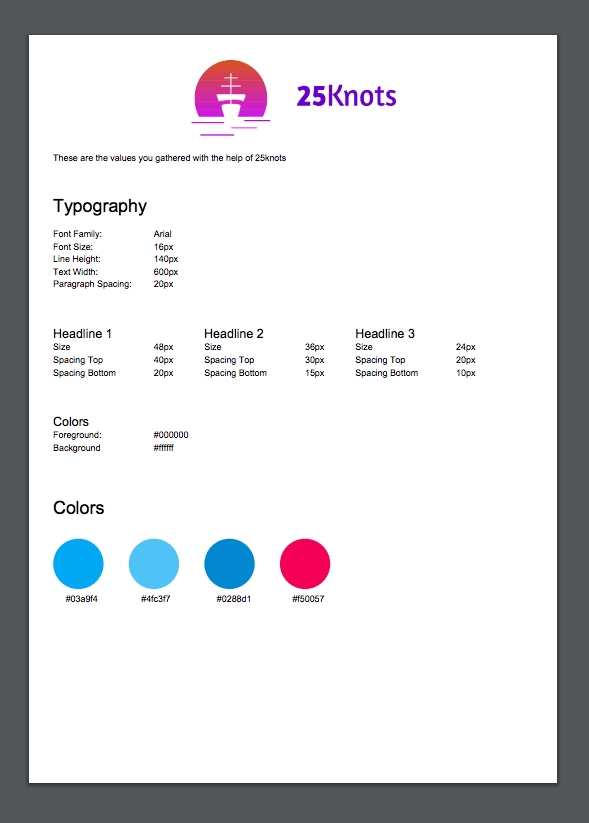
\includegraphics[width=0.4\textwidth]{images/pdf_generated.png}
    \caption{Beispiel einer generierten PDF-Datei}
    \label{fig:pdf}
\end{figure}
